\section{The GreenMeasurer Framework}
\label{sec:greenmeasurer}

GreenMeasurer is a framework developed to support the measurement of software energy consumption using the hardware energy counters exposed by CPUs and GPUs. It automates the configuration, execution and collection of energy metrics, aiming to make energy profiling practical and reproducible for software developers and researchers. It runs on Linux (Intel CPUs and integrated GPUs, NVIDIA GPUs) and macOS (Apple Silicon).

\subsection{Overview}

The framework combines a set of Bash scripts, C utilities and Makefiles to form a reproducible measurement pipeline that requires minimal user intervention; it does not require modifying source code to measure the energy consumption of a program.

The general architecture is shown in Figure~\ref{architecture_diagram}, which illustrates the workflow of the framework. First, the framework is executed with the appropriate arguments configured for the experiment. The next step is \textit{CPU temperature calibration}: the system is left idle for a specified number of seconds (it is executed a \textit{sleep} command), during which the average temperature of all CPU cores is recorded using the \textit{lm-sensors} library \cite{lm-sensors} and stored in a text file. Optionally, a \textit{power cap calibration} can be performed. In this step, a custom program (for example, the provided Python implementation of the Fibonacci algorithm) is executed across a range of power caps. A Python script then analyzes the resulting CSV file to identify the optimal power cap, defined here as the value that minimizes \textit{Package} energy consumption. After calibration, the framework can perform either over-time measurements or standard repeated executions. In the over-time mode, the target program is executed while continuously logging, at a user-defined interval, the energy metrics of the selected backends along with CPU temperature. In the standard mode, the framework first performs a series of idle runs for a specified number of seconds (executes a \textit{sleep} command), repeated \textit{n\_times} times, to establish the baseline energy consumption of the system under minimal load. Only after completing these idle measurements is the target program executed, with all results appended to the CSV file \texttt{measurements.csv}. The purpose of the idle runs is to isolate the program's energy consumption from the system's baseline energy usage. Each entry in this CSV file starts with the fields below, followed by one column per metric declared by the selected backends (named \texttt{<category>.<name>\_<unit>}, Table~\ref{table:metrics}):

\begin{itemize}
    \item \textbf{Language} - Programming language label (text).
    \item \textbf{Program} - Program name label (text).
    \item \textbf{Powercap} - Power cap value applied (W), or $-1$ if none.
    \item \textbf{Time\_ms} - Execution time (ms).
    \item \textbf{CPU\_Memory\_KB} - Peak resident memory of the command (KiB), measured in a separate run.
\end{itemize}

An unavailable value is written as \texttt{NOT\_SUPPORTED}, never as zero.

\begin{figure*}[!ht]
    \centering
    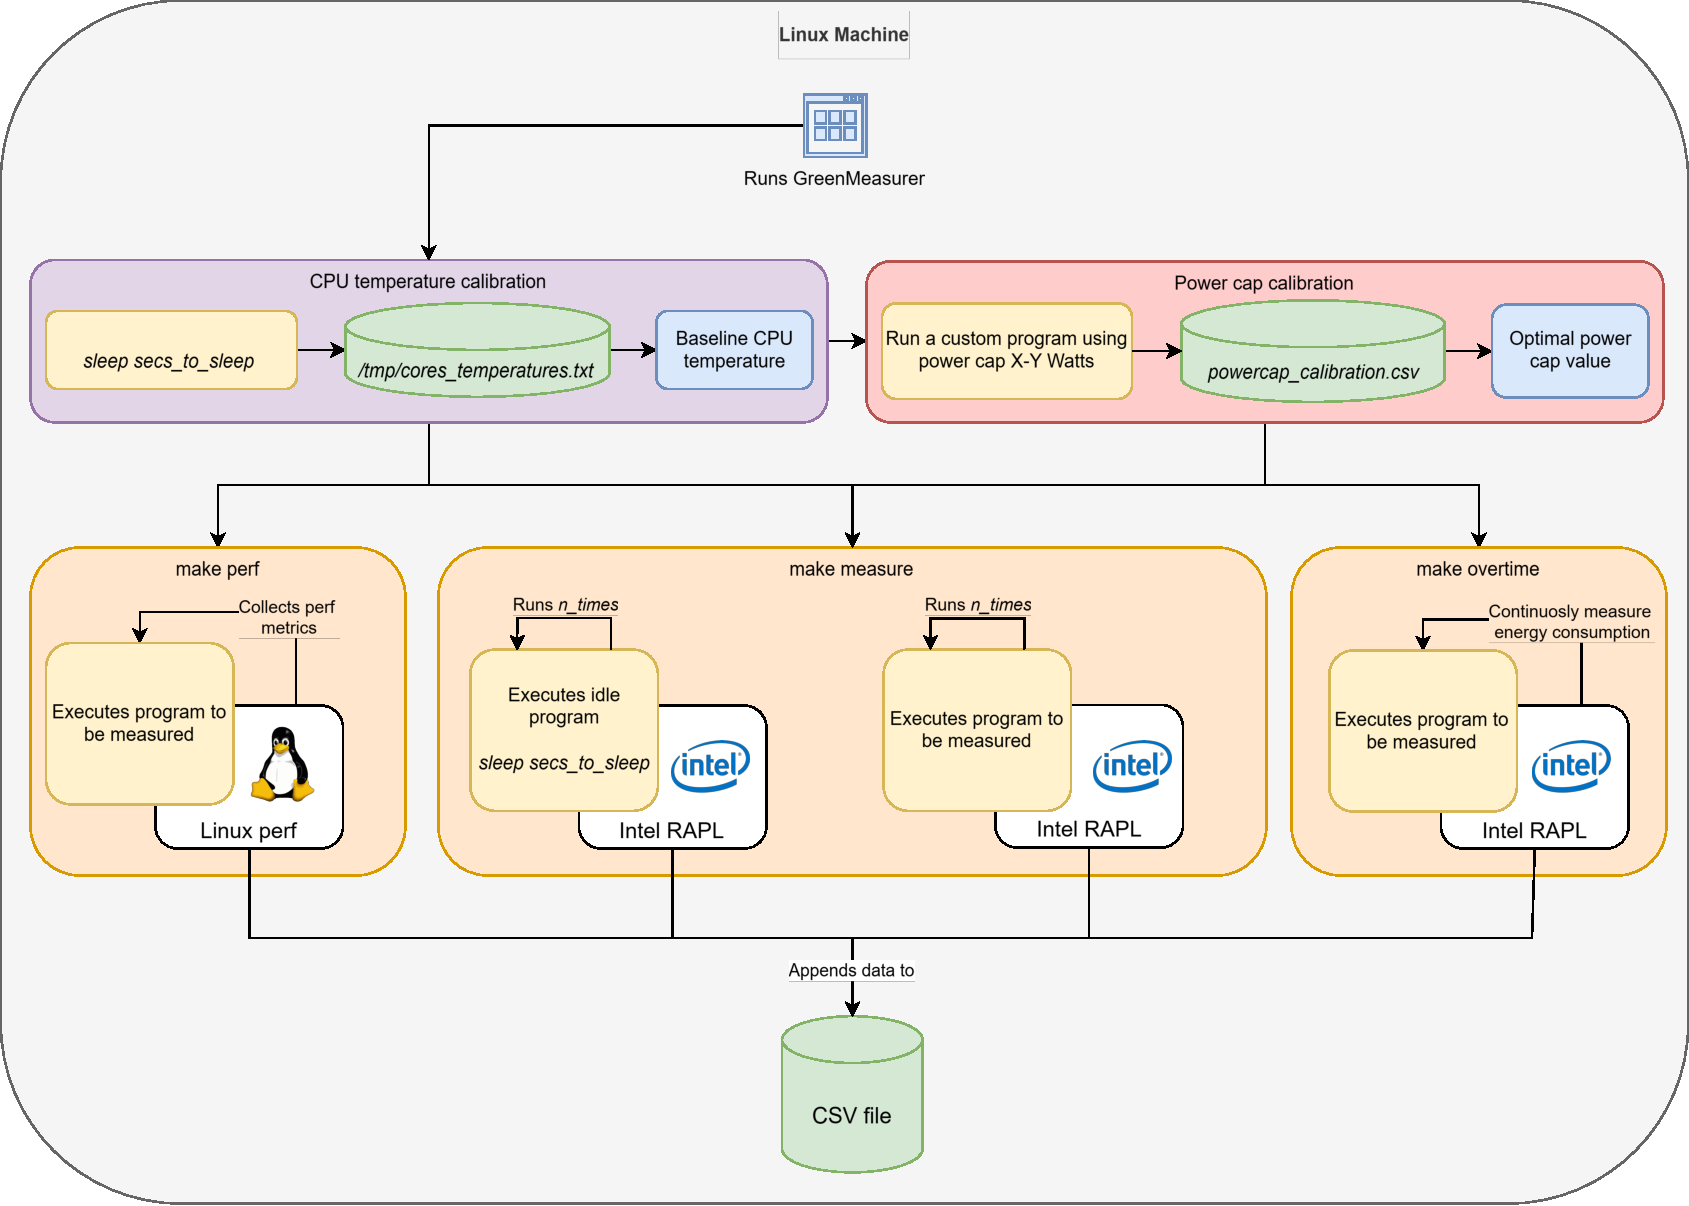
\includegraphics[width=\linewidth]{images/architecture.pdf}
    \caption{GreenMeasurer Architecture}
    \label{architecture_diagram}
\end{figure*}

In Table \ref{table:arguments}, we present the parameters of \textit{GreenMeasurer}, many of which are shared by the \textit{standard} mode, \textit{over-time} measurements (Section~\ref{overtime_section}) and the two calibration modes (Section~\ref{calibration_modes_section}).

\begin{table*}[t]
    \centering
    \caption{Command-line options of GreenMeasurer. All modes accept \texttt{-command} (the command to run through \texttt{/bin/sh -c}).}
    \label{table:arguments}
    \small
    \begin{tabularx}{\textwidth}{@{}l l l X@{}}
        \toprule
        \textbf{Option} & \textbf{Unit/type} & \textbf{Modes} & \textbf{Meaning} \\
        \midrule
        \texttt{-language} & text & all & Label written to the \texttt{Language} column; it does not change how the command runs. \\
        \texttt{-program} & text & all & Label written to the \texttt{Program} column. \\
        \texttt{-n\_times} & count & std.\ (1), cal.\ (3) & Number of measured runs (per power limit in calibration). \\
        \texttt{-variance} & \si{\celsius} & all & Maximum temperature above the calibrated baseline at which a run may start; otherwise the tool waits, checking every second (defaults: 0 standard, 5 over-time and calibration). Skipped if no CPU temperature is available. \\
        \texttt{-time\_out\_limit} & hours & std., cal. & Time limit of the initial check run; on expiry a \texttt{TimeOut} row is recorded (default 1). \\
        \texttt{-interval} & ms & over-time & Time between samples (default 100). \\
        \texttt{-powercap} & W, or $-1$ & std., over-time & Package power limit (Intel only); $-1$ means no cap (default); otherwise at least 1. \\
        \texttt{-sleep\_time}, \texttt{-sleep-secs} & s & all & Idle time used to settle the machine when a temperature baseline has to be created (default 5; 10 as \texttt{-secs\_to\_sleep} in calibration). \\
        \texttt{-calib-file} & path & all & Baseline-temperature file (default \texttt{/tmp/cores\_temperatures.txt}). \\
        \texttt{-output} & path & all & Output CSV (defaults \texttt{measurements.csv}, \texttt{measurements\_ot.csv}, \texttt{powercap\_calibration.csv}). \\
        \texttt{-range} & \texttt{min-max}, W & cal. & Range of power limits to test; the minimum is 1 W. \\
        \texttt{-compile\_cmd} & text & cal. & Optional command run once before the sweep. \\
        \bottomrule
    \end{tabularx}
\end{table*}

\begin{table*}[t]
    \centering
    \caption{Output metrics. A \emph{window} metric is the difference of a counter between the start and the end of the run (cumulative since the start in over-time mode); a \emph{gauge} is a single reading; a \emph{peak} is the highest reading seen while the command ran.}
    \label{table:metrics}
    \small
    \begin{tabularx}{\textwidth}{@{}l l l l X@{}}
        \toprule
        \textbf{Column} & \textbf{Unit} & \textbf{Kind} & \textbf{Backend} & \textbf{Meaning} \\
        \midrule
        \texttt{Time\_ms} & ms & core & all & Duration of the run (\texttt{Timestamp\_ms}: time since start, in over-time mode). \\
        \texttt{CPU\_Memory\_KB} & KiB & core & all & Peak resident memory of the command (separate run). \\
        \texttt{cpu.Package\_J} & J & window & Intel & Energy of the CPU package. \\
        \texttt{cpu.Core\_J} & J & window & Intel & Energy of the cores (part of the package). \\
        \texttt{cpu.DRAM\_J} & J & window & Intel & Energy of the memory. \\
        \texttt{cpu.Temperature\_C} & \si{\celsius} & gauge & Intel & Average core temperature. \\
        \texttt{cpu.CPU\_J}, \texttt{cpu.ANE\_J} & J & window & Apple & CPU and Neural Engine energy from \texttt{powermetrics}. \\
        \texttt{gpu.GPU\_J} & J & window & NVIDIA, Intel, Apple & GPU energy. \\
        \texttt{gpu.Power\_W} & W & gauge & NVIDIA & Instantaneous GPU power. \\
        \texttt{gpu.Temperature\_C} & \si{\celsius} & gauge & NVIDIA, Intel & GPU temperature. \\
        \texttt{gpu.Utilization\_\%} & \% & gauge & NVIDIA & GPU utilization. \\
        \texttt{gpu.VRAM\_MiB} & MiB & peak & NVIDIA & GPU memory used by the process. \\
        \bottomrule
    \end{tabularx}
\end{table*}

\subsection{Backends}
\label{sec:backends}

The core (\texttt{main.c}) handles the command line, orchestration, sampling, calibration and CSV output, and contains no hardware-specific code. Hardware support lives in \emph{backends}: shared objects (\texttt{backend.so}) placed under \texttt{platform/<os>/cpu/<name>} or \texttt{platform/<os>/gpu/<name>}. At startup the core loads each \texttt{backend.so}, validates its exported descriptor, calls its \texttt{detect()} function, and selects the detected backend with the highest priority in each category. One CPU backend and one GPU backend are chosen independently. If a category has no usable backend, its metrics are written as \texttt{NOT\_SUPPORTED} and the run continues; only when neither category is usable does the tool exit with an error. The backend directory can be overridden with \texttt{GREENMEASURER\_BACKEND\_DIR}, and \texttt{GREENMEASURER\_VERBOSE\_BACKENDS=1} lists the state of every backend (\texttt{selected}, \texttt{available}, \texttt{not detected}, \texttt{not built}, \texttt{load failed}, \texttt{invalid}). Table~\ref{table:backends} lists the existing backends.

\begin{table}[t]
    \centering
    \caption{Backends in the repository.}
    \label{table:backends}
    \small
    \begin{tabularx}{\columnwidth}{@{}l l X@{}}
        \toprule
        \textbf{Type} & \textbf{Backend} & \textbf{Source / status} \\
        \midrule
        CPU & Intel & RAPL MSRs; temperature; power capping \\
        CPU & AMD Zen & MSRs; not validated, future work \\
        CPU & Apple Silicon & \texttt{powermetrics}; not yet validated \\
        GPU & Intel integrated & RAPL PP1 MSR \\
        GPU & NVIDIA & NVML total-energy counter \\
        GPU & Apple Silicon & \texttt{powermetrics}; not yet validated \\
        \bottomrule
    \end{tabularx}
\end{table}

\subsection{Adding a Backend}
\label{sec:adding_backend}

A backend implements the interface in \texttt{energy-backend.h}: a \texttt{detect} function, \texttt{init}/\texttt{cleanup}, \texttt{sample\_start}/\texttt{sample\_stop} (the measurement window), a table of metric descriptors (name, unit, kind and scope) and a \texttt{get\_metric} function, plus an exported \texttt{energy\_backend\_descriptor} with its category and priority. Power capping is optional for CPU backends. The repository includes two complete, working examples, TOY\_CPU and TOY\_GPU (in \texttt{examples/toy\_backends}), whose energy values are fake by design. TOY\_CPU declares \texttt{cpu.Energy\_J} (window) and \texttt{cpu.LoadAvg\_1m} (gauge); TOY\_GPU declares \texttt{gpu.Energy\_J}, \texttt{gpu.Power\_W} and \texttt{gpu.Memory\_MiB}. Each is a single C file of about one hundred lines, built with \texttt{make -C examples/toy\_backends} and loaded without touching the core by setting \texttt{GREENMEASURER\_BACKEND\_DIR}. Moving the directory into \texttt{src/platform/} makes the standard build pick it up. The CSV columns of the new metrics appear automatically.

\subsection{System Requirements}

GreenMeasurer runs on Linux and on macOS (Apple Silicon). The \texttt{src/Makefile} selects \texttt{platform/linux} or \texttt{platform/macos} according to the operating system. Reading the energy counters requires root privileges. On Linux the Intel backends use RAPL through the \texttt{msr} kernel module; CPU temperature is read with \textit{lm-sensors} \cite{lm-sensors}; the Intel power-capping support uses \textit{powercap} \cite{powercap2025} and \textit{raplcap} \cite{raplcap}; the NVIDIA backend needs the NVML header and library at build time. A missing optional dependency only skips the backend that needs it. On macOS there are no RAPL or MSR counters, so the Apple backends run \texttt{powermetrics} in the background and integrate the average power it reports in each sampling interval (100 ms by default) into energy; the energy is thus known only to within one sampling interval. There is no power capping and no CPU temperature on macOS. The helper scripts that disable Wi-Fi are Linux-only. On Linux, a dedicated setup script installs the dependencies (\textit{i.e.} \textit{raplLibrariesSetup.sh}).

\subsection{Makefile Integration}

To evaluate a software system, a dedicated \textit{Makefile} must exist that defines a common set of targets for compilation, execution and measurement. This structure provides a uniform interface across heterogeneous environments and simplifies experiment automation.

The standard targets are:
\begin{itemize}
    \item \texttt{compile} - builds the program using the corresponding compiler or interpreter;
    \item \texttt{run} - executes the compiled or interpreted program with a parametrized input;
    \item \texttt{standard} - runs the program and collects energy and runtime data with the selected backends;
    \item \texttt{overtime} - runs the program and collects energy data with the selected backends during the program's execution time (see Section \ref{overtime_section});
    \item \texttt{clean} - removes all generated binaries and temporary files.
\end{itemize}

This Makefile-based design ensures consistent measurement behavior across all programs, allowing researchers to reproduce experiments by invoking the same target. 

\subsection{Calibration Modes}
\label{calibration_modes_section}

To improve the reliability of the collected data, GreenMeasurer supports two calibration modes.

The \textit{temperature calibration} mode measures the average temperature of CPU cores by executing a \textit{sleep} command for a specified number of seconds (\textit{secs\_to\_sleep} argument from Table \ref{table:arguments}). It then records the average temperature of all cores using the \textit{lm-sensors} library. Whenever a program is about to run, the CPU temperature must be below or equal to the baseline temperature plus a user-defined temperature variance (\textit{variance} from Table \ref{table:arguments}), otherwise a \textit{sleep} command of one second is executing until the condition is met. This mode can be executed as follows:

\begin{verbatim}
sudo ./main --temperature-calibration -sleep-secs 20
\end{verbatim}

The \textit{power cap calibration} mode iteratively tests different power cap values to determine the most energy-efficient setting (least \textit{Package} energy consumption) for a given workload. Power capping is available only on Intel CPUs, and the tool validates this at run time: if the selected CPU backend has no power-capping support (e.g., no Intel CPU), calibration and capped runs abort with an error instead of silently running uncapped. Power capping has been used in previous studies \textbf{[cite]}. Users provide a custom program for testing - for example, the GreenMeasurer repository includes a recursive Fibonacci algorithm in Python located in the \texttt{Utils/} folder. This mode can be executed as follows (where \textit{min} and \textit{max} define the range of power cap values, \textit{compile\_cmd} is the compilation command for the custom program - omit if using an interpreted language - and \textit{run\_cmd} is the execution command):

Both calibration modes are designed to make energy measurements more reproducible. The temperature calibration ensures similar CPU conditions across runs, while power cap calibration automatically finds the most efficient power limit for a certain system. This combination helps minimize measurement noise and allows consistent comparisons across experiments.

\begin{verbatim}
sudo ./main --powercap-calibration -range <min>-<max>
     -variance <variance> -time_out_limit <hours>
     -secs_to_sleep <s> -n_times <n>
     [-compile_cmd <cmd>] -command <run_cmd>
     -language <language> -program <program>
\end{verbatim}


\subsection{Over-Time Measurements}
\label{overtime_section}

This section describes an execution mode of \textit{GreenMeasurer} called \textit{over-time measurements}. In this mode, the target program is executed while the backends are sampled at regular intervals. The energy consumption reported by the selected backends is then recorded into a CSV file named \texttt{measurements\_ot.csv}. We recommend using the smallest possible interval to obtain more fine-grained measurements throughout the program's runtime.

Additionally, the CPU temperature is recorded immediately before each measurement interval and stored in the same CSV file. The number of entries in the file corresponds to the total number of intervals executed.

The tool can be executed as follows, where \textit{interval} specifies the measurement interval in milliseconds and the remaining arguments are described in Table~\ref{table:arguments}:

\begin{verbatim}
sudo ./main --overtime -command <command>
     -interval <ms> -language <language>
     -program <program> -powercap <W>
     -sleep-secs <s> -variance <C>
\end{verbatim}


\subsection{Measurement Pipeline}

An automated and simplified way to run \textit{GreenMeasurer} on Linux is illustrated in Figure~\ref{measure_sh_diagram}, which shows the measurement process coordinated by the main script \texttt{measure.sh}. On macOS the executable or the workload Makefiles are used directly.

First, the script disables the Wi-Fi interface (the user must identify the correct interface name). It then builds the framework, including the core and the available backends. 

After this setup, for each program in each programming language to be analyzed, and for each power cap value to be tested, the script compiles the program and executes the corresponding measurement procedure - either \textit{measure} or \textit{over-time} (Section~\ref{overtime_section}).

\begin{figure*}[!ht]
    \centering
    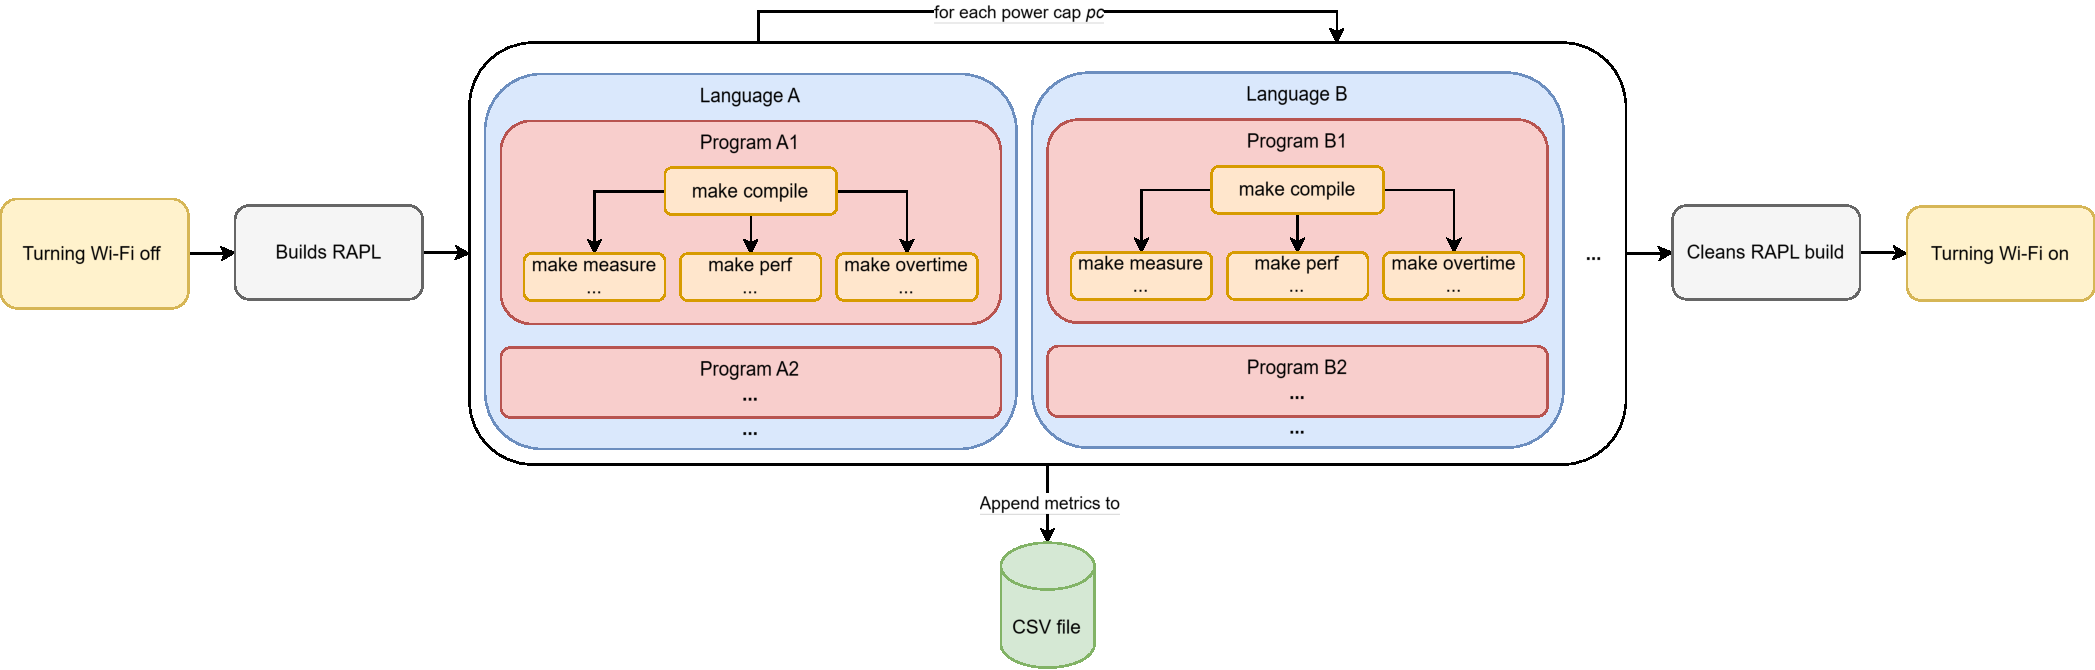
\includegraphics[width=\linewidth]{images/measure_sh.pdf}
    \caption{Running GreenMeasurer through the \texttt{measure.sh} script.}
    \label{measure_sh_diagram}
\end{figure*}

To prevent the need for manual system recovery, \textit{GreenMeasurer} automatically restores Wi-Fi and power settings after each measurement or if the process is interrupted.
